\section{PMAC Motor}\label{sec:PMAC} %by Martin

%\subsection{Requirements}
%\subsection{Analysis}
%\subsection{Conclusion}
This section focuses on the motor used for this project.
Initially the functionality of the motor will be described, then certain motor parameters will be tested, as the online product description is not all that clear.
Lastly a parking test will be performed to determine the angle of the encoder mounted on the motor. 
The motor used to drive the go-kart is an 8-pole non-salient permanent magnet synchronous motor. 

\subsection{Motor description}\label{sub:motor_descrpition}
The motor used is a 3-phase Wye-connected, 8-pole non-salient permanent magnet AC motor, the Motenergy ME1117.
Although there are many different types of PMAC motors, there is no physical difference between brushless DC motors (BLDC), permanent magnet AC motors (PMAC), and permanent magnet synchronous motors (PMSM). 
The motor will be driven as an AC or synchronous motor (since these are the same) to produce a more consistent torque.
This means that the rotor consists of four pairs of magnets - one with the north side facing outward towards the stator and one with the north side facing inward to the ferromagnetic core of the rotor. 
The stator consists of 24 solenoids mounted inward on a ferromagnetic outer ring. 
Looking at the motor from the axle side, a counter clockwise rotoration results in the go-kart going forward. See figure~\ref{fig:motor_24p}.
The solenoids are placed so that the four phase A solenoids are placed along the horizontal and vertical axes - this is not necessarily true, but a parking test will be performed in section~\ref{sub:parking_test} to determine the actual placement.
The order of the other solenoids, when going counter-clockwise is then $\bar{B}$, $C$, $\bar{A}$, $B$ and $\bar{C}$, as shown on figure~\ref{fig:motor_24p}. 
The solenoids $A$ correspond to terminal M1, solenoids $B$ correspond to M2, and solenoids $C$ correspond to M3. 
Current going into terminal M1, will then pass through all the $A$ and $\bar{A}$ solenoids in series, before reaching the star point, and continuing through $B$ and $\bar{B}$ and/or $C$ and $\bar{C}$.

\begin{figure}[H]
	\begin{center}
		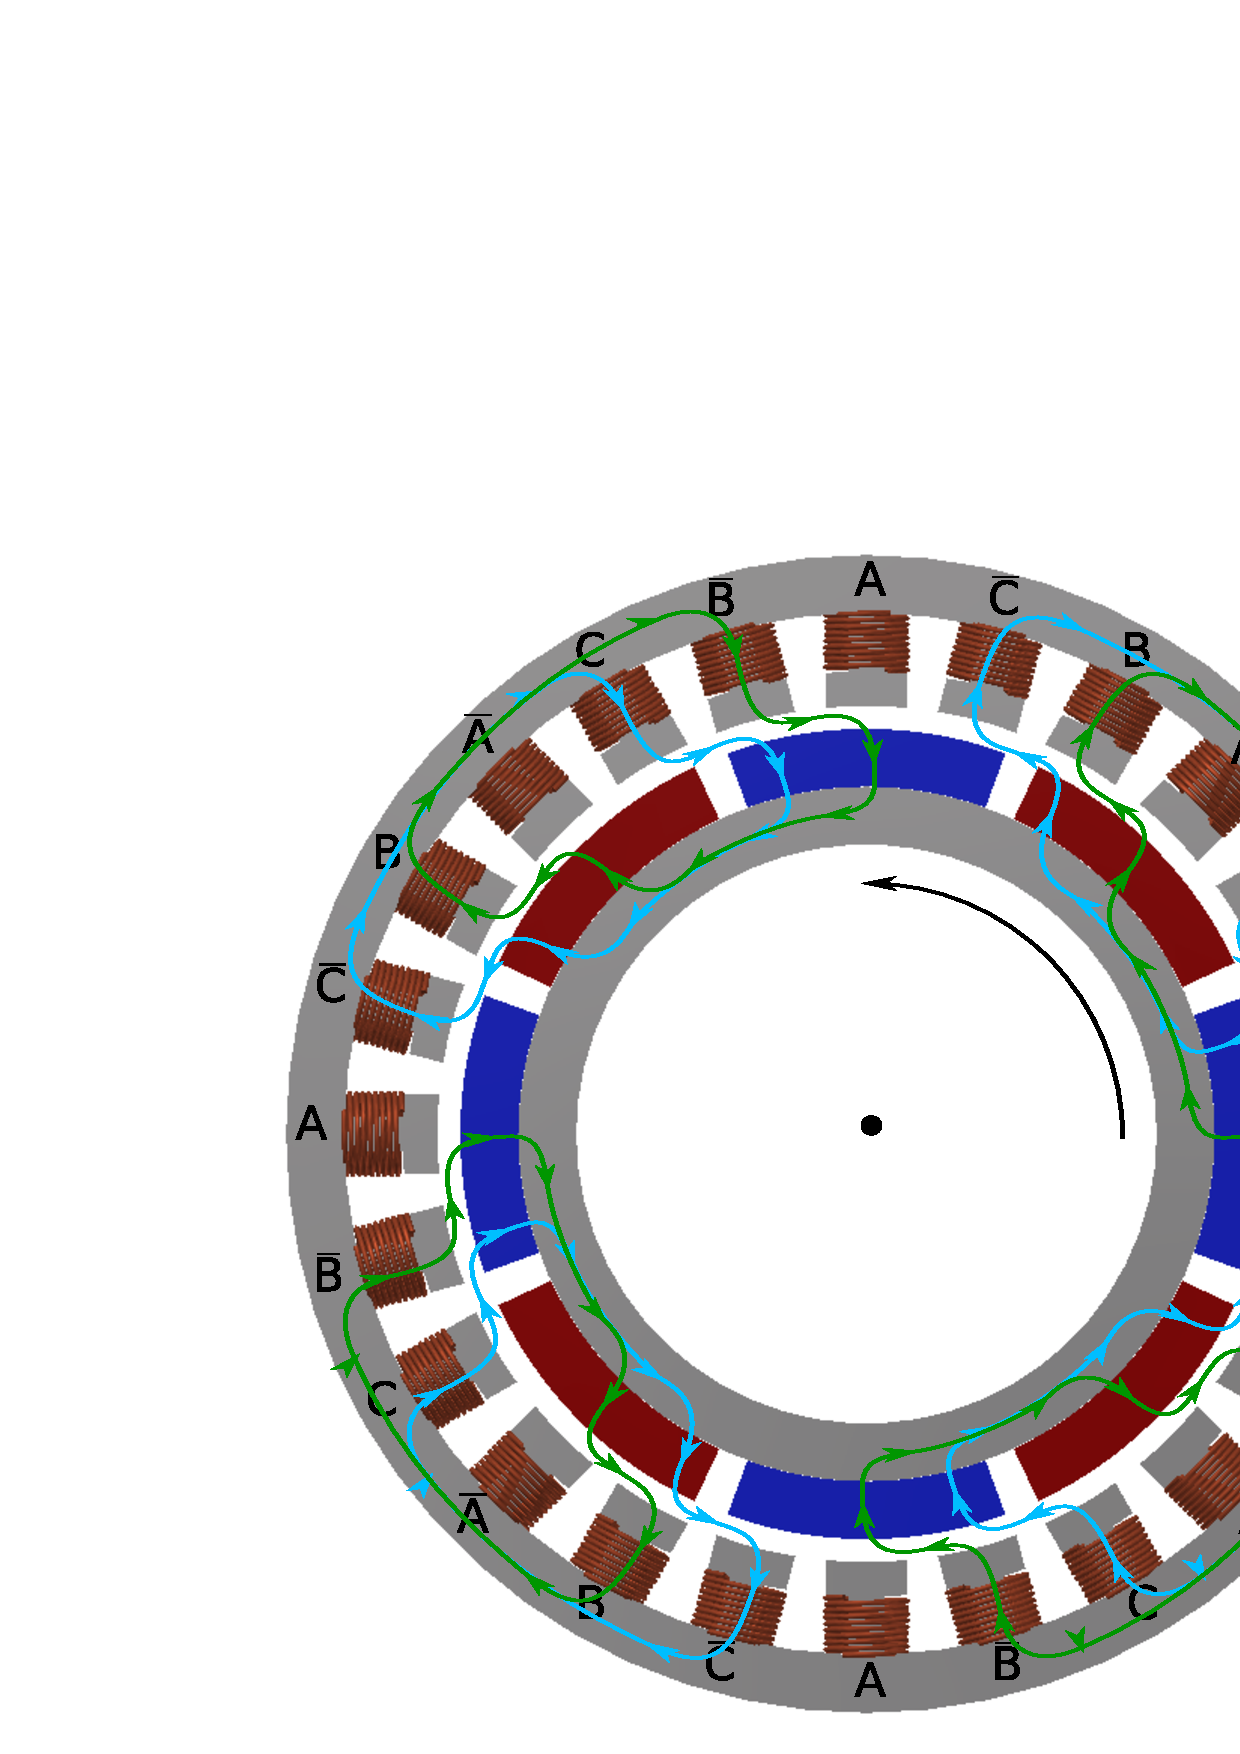
\includegraphics[width=.75\linewidth]{graphics/motor_24p_sketch}
		\caption[Cross section diagram of the motor.]{Cross section diagram of the motor. Magnetic flux lines are drawn in green and cyan for a stator field being 90 electrical degrees ahead of the rotor.}
		\label{fig:motor_24p}
	\end{center}
\end{figure}

According to the manufacturer, the motor is rated for 48VDC and up to 300A for a minute. This corresponds well with its 19hp rating, which means, this DC voltage is the input voltage when driving it as a brushless DC motor, and thus a DC supply voltage of 52.8V does not overload the motor.
However, due to limitations on the power rail the power peaks at 14.7hp.
This happens when equation~\ref{eq:max_power_velocity} is true.
\begin{equation}
V_{BEMF} = \frac{V_{bat}}{2} - I_{max} \cdot R_a
\label{eq:max_power_velocity}
\end{equation}
Using $K_E$ as defined in equation~\ref{eq:KE_definition} to convert the back EMF voltage into a velocity, the maximum power is reached at 3186rpm.
For controlling the motor it can be considered a 2-pole motor, which means that there are only two magnetic fields; the rotor magnetic field generated by the permanent magnets, and the stator field generated by the solenoids. 
This is achieved by converting the measured mechanical angle of the rotor to electrical angle, and then doing all calculations in this domain.

\begin{figure}[H]
	\begin{center}
		\includegraphics[width = .35\linewidth]{graphics/motor_6p}
		\caption{Simplified motor model showing the stator field as green arrows}
		\label{fig:motor_6p}
	\end{center}
\end{figure}

The electric angle of figures~\ref{fig:motor_24p} and~\ref{fig:motor_6p} are the same, and the stator field is set 90 degrees ahead. 
In figure~\ref{fig:motor_6p}, the rotor magnet will always try to line up with the magnetic field lines. 
In the real motor, this will cause the magnetic path to become shorter, as the rotor lines up the permanent magnet poles with the opposite pole of the solenoids. 
By constantly placing the stator field ahead of the rotor, the motor will start moving.
Thus it is necessary to know the position of the rotor in order to determine the angle of the stator field.
For that measurement, an encoder will be used.

\subsection{Definition of Back-EMF Constant and Torque Constant}
The parameters $K_E$ and $K_T$ must be the same for a PMAC motor, since they are dependent on the flux produced in the permanent magnet of the rotor. 
Another reason, that they are the same is, that the motor converts electrical energy to mechanical energy, and electrical energy is the product of current and voltage, and (rotational) mechanical energy is the product of torque and angular velocity. 
A mismatch between $K_E$ and $K_T$ implies, that power appears or disappears, which cannot happen. 

The Back-EMF constant, $K_E$, is defined as the amplitude of each phase-voltage divided with the mechanical angular velocity.

\begin{eqnarray}
K_E =& \frac{V_{BEMF}}{\omega _m}\\
K_T =& \frac{T}{1.5\cdot I_q}
\label{eq:KE_definition}
\end{eqnarray}
This means that $K_E$ and $K_T$ are the same, and the torque produced is the q-current multiplied by $K_T$ and 1.5.
The mathematical reasoning behind is explained by power conservation in equations~\ref{eq:power_electrical_mechanical} through~\ref{eq:mechanical_power_from_electrical}, and by torque contribution in equations~\ref{eq:torque_contributions} through~\ref{eq:torque_function_90deg}. \\

Consider an ideal motor producing some torque, T, and running at a constant angular velocity, $\omega$. 
Losses in the armature resistance and friction are zero. 
The motor is driven by a quadrature current, $I_q$, and a quadrature voltage, $V_q$. 
Currents and voltages along the d-axis are 0. 
The electrical power going into the machine must be equal to the mechanical power going out:

\begin{equation}
P_m = P_e
\label{eq:power_electrical_mechanical}
\end{equation}

Mechanical power is the product of torque and angular velocity:

\begin{equation}
P_m = \omega T
\label{eq:power_mechanical}
\end{equation}

Since there is no phase difference between voltages and currents, electrical power is the product of the RMS values of the current and voltage per phase, times 3:

\begin{equation}
P_e = 3\Big(\frac{1}{\sqrt{2}}V \cdot \frac{1}{\sqrt{2}}I \Big) = V \cdot \frac{3}{2} I
\label{eq:power_electrical_RMS}
\end{equation}

The angular velocity and torque can be calculated from the voltage and current, respectively, and put into equation \ref{eq:power_mechanical}:

\begin{equation}
P_m = \Big( \frac{V}{K_E} \Big) \cdot \big( \frac{3}{2} I \cdot K_T \big)
\label{eq:mechanical_power_from_electrical}
\end{equation}

By setting $K_E = K_T$, equations~\ref{eq:power_electrical_RMS}~and~\ref{eq:mechanical_power_from_electrical} yield the same. \\

Hence, a factor of 1.5 is multiplied to $V\cdot I$ to get the mechanical power. This factor is tied to $K_T$: \\
Consider a motor with with an optimal controller, so the d-current is zero, and the q-current is I. 
The phase current is then calculated by:

\begin{equation}
\begin{bmatrix}
I_a \\ I_b \\ I_c
\end{bmatrix}
=
\begin{bmatrix}
I \cdot \cos(\theta _f) \\ I \cdot \cos(\theta_f - \gamma) \\ I \cdot \cos(\theta_f + \gamma)
\end{bmatrix}
\label{eq:current_q}
\end{equation}

where $\theta_f$ is the electrical angle of magnetic field generated by the stator, and $\gamma = \tfrac{2 \pi}{3}$. In this case, the motor is at constant speed, so the amplitude of all currents are the same.\\
Each of the three phases then contribute to the total torque, depending on the angle between the rotor and the phase, calculated by:

\begin{equation}
\begin{bmatrix}
T_a \\ T_b \\ T_c
\end{bmatrix}
=
\begin{bmatrix}
-I_a \cdot K_T \cdot \sin(\theta _r) \\ -I_b \cdot K_T \cdot \sin(\theta_r - \gamma) \\ -I_c \cdot K_T \cdot \sin(\theta_r + \gamma)
\end{bmatrix}
\label{eq:torque_contributions}
\end{equation}

where $\theta_r$ is the electrical angle of the rotor. \\

The total torque is then the sum of the torque contribution of each phase: 

\begin{equation}
T = T_a + T_b + T_c
\label{eq:total_torque_contribution}
\end{equation}

The torque produced as a function of the angle difference can be calculated with equation~\ref{eq:torque_fucntion_angle}:

\begin{equation}
T(d\theta) = \frac{3}{2} I \cdot K_T \cdot sin(d\theta)
\label{eq:torque_fucntion_angle}
\end{equation}

This can be verified by inspection of figure \ref{fig:torque_contribution_dphi}.
The rotor angle is fixed at 45\si{\degree}. 
$\theta_f$ will go from -135 degrees to 225 degrees. 
Figure~\ref{fig:torque_contribution_dphi} shows torque contribution from each of the three phases, where I and $K_T$ are 1.

\begin{figure}[H]
	\centering
	\includegraphics[width = 10cm]{graphics/torque_contribution_dphi}
	\caption{Torque contribution of each phase as a function of the phase difference}
	\label{fig:torque_contribution_dphi}
\end{figure}
	
	Adding these three contributions gives equation~\ref{eq:torque_fucntion_angle}.
	
	If $d\theta = 90 \si{\degree}$, equation~\ref{eq:torque_fucntion_angle} becomes:
	
\begin{equation}
	T = \frac{3}{2}K_t \cdot I
	\label{eq:torque_function_90deg}
\end{equation}
	
It is easier to measure $K_E$ than $K_T$ and they are defined as the same. \\

\subsection{Motor Parameterization}\label{sub:1117_param}
Due to the sparse information available from the manufacturer of the motor, it is necessary to measure some of the parameters of the motor. 
It will also be necessary to determine exactly what these parameters define, since the manufacturer has not defined certain things such as what current measurement is related to torque through $K_T$.
Parameters to determine are the back-EMF constant, $K_E$, the armature resistance, $R_a$, and the armature inductance, $L_a$.
Each of the following sections describe the procedure used to find each of these parameters. 

\subsubsection{Measuring Back-EMF Constant}\label{sub:KE-KT}
To find $K_E$, a hand-held power drill is used to rotate the motor at a constant speed. 
An oscilloscope with a differential probe is used to measure the voltage between two of the phases. 
Because of the high input impedance of the differential probe, there is no current and thus the armature inductance and resistance can be neglected. 
The peak-peak voltage and the corresponding frequency is noted in the table below:

\begin{table}[!h]
\begin{center}
\begin{tabular}{S|S}
	{Frequency }[\si{\hertz}]  & {Voltage } [\si{\volt}$_{\text{pp}}$] \\
	\hline
	23.49 & 9.7  \\
	38.32 & 15.3\\
	40.97 & 16.5\\
	44.9 & 17.7\\
	54.7 & 21.8\\
	61.81 & 24.2\\
	72.13 & 28.3
\end{tabular}
\end{center}
\caption{Measured line-line voltage at electrical frequencies}
\label{tab:KE_measurements}
\end{table}

The phase amplitude of the voltage is calculated by dividing the voltages in table~\ref*{tab:KE_measurements} with $2\sqrt{3}$. The mechanical angular velocity is calculated by multiplying the frequency in table~\ref*{tab:KE_measurements} with $2\pi$, and dividing with $4$ pole pairs. 
The resultant voltages and velocities are divided to calculate $K_E$, and the average is calculated for these. 
The result is:

\begin{equation}\label{eq:K_E}
K_E = K_T = 0.0733 \si{\volt\second\per\radian}
\end{equation}

with a spread of 1.3\%. 
According to the datasheet, $K_T$ is 0.13. 
This is 1.77 times higher than the measured $K_E$. 
There are two potential reasons for this.
One is, that the manufacturer uses line-to-line currents and voltages instead, since the difference is close to $\sqrt{3}$. 
Another possible reason is, that the manufacturer defines $K_T$ as the torque produced with the given q-current, in which case $K_T = 1.5K_E$, and the measured $K_T$ is about 15\% below the manufacturer's datasheet. 
Whatever the reason, equation~\ref{eq:K_E} will be used throughout this report. \\

This means, the maximum speed and torque can be calculated:

\begin{equation}
\omega _{max} = \frac{V_{bat}}{2 K_E} = 360 \si{\radian \per \s} 
\label{eq:max_rotational_speed}
\end{equation}

\begin{equation}
T_{max} = I_{max} \cdot \frac{3}{2} K_T = 33 Nm
\label{eq:max_torque}
\end{equation}

\subsubsection{Armature Resistance}\label{sub:R_a-measurements}
To measure the armature resistance, a high DC current is driven through one terminal to the other. 
The voltage at the terminal is measured.
The large current causes a significant voltage drop in the wires leading from the power supply to the motor. 
Based on the measured voltages and currents the resistance between the two terminals can be calculated.
The results are shown in the table below:

\begin{table}[h]
	\begin{center}
	\begin{tabular}{r | c | c | c}
		{Terminals} 	& {V} [\si{\volt}]	& {I} [\si{\ampere}]	& {R} [\si{\milli\ohm}] \\
		\hline
		{AB} 			& 0.217 		& 17.93 		& 12.10  \\
		\hline
		{AC}			& 0.206  		& 17.96 		& 11.47  \\
		\hline
		{BC}			& 0.235 		& 17.93  		& 13.11
	\end{tabular}
	\end{center}
	\caption{Measured DC resistance across terminal-pairs.}
	\label{tab:armature_resistance}
\end{table}

It is desirable to know the resistance from one terminal to the common star point. 
That can be calculated by equation~\ref{eq:resistance_converter}

\begin{equation}
R_a = \frac{R_{AB} + R_{AC} - R_{BC}}{2}
\label{eq:resistance_converter}
\end{equation}

This gives different armature resistances for different phases ranging from 5.2 to 6.9 \si{\milli\ohm}. 
This is about half the line-to-line resistance listed by the manufacturer at 13\si{\milli\ohm}. 
However, since the motor is a wye connection, knowing the resistance between a terminal and the star-point is more helpful when modeling the motor.

\subsubsection{Armature Inductance}\label{sub:L_A-measurements}
In order to measure the winding inductance of the motor, a full bridge driver is used to generate a square wave at different frequencies. 
The two terminals of the full bridge driver is connected to terminals B and C, and voltage and current is measured.
The motor is not moving, so there is no back-EMF. 
The resistor voltage is subtracted from the voltage measurements, and what remains is the inductor voltage. 
Current and voltage has been plotted in figure~\ref{fig:20kHz_squarewave}.  

\begin{figure}[H]
	\begin{center}
		\includegraphics[width = 10cm]{graphics/inductance_measured_v_i}
		\caption{20 kHz square wave voltage and the resulting current.}
		\label{fig:20kHz_squarewave}
	\end{center}
\end{figure}

These waveforms have been measured at 5 kHz, 10 kHz, 20 kHz and 30 kHz. 
For this project a switching frequency of 20 kHz will be used, so only this plots will be shown. 
Due to the high sampling rate of the oscilloscope and low bit resolution, differentiating the current will yield very large spikes for short periods of time. 
Therefore, the current, time and voltage measurements will be periodically averaged and downsampled by a factor of 70. 
The derivative of the current is then calculated by:

\begin{equation}
\frac{di}{dt}[n] = \frac{i[n]-i[n-1]}{t[n]-t[n-1]}
\end{equation}

This is the derivative of the current at the point immediately between two samples, so to synchronize the time and voltage arrays, each two consecutive samples are averaged. 
The resulting waveforms are plotted in figure~\ref{fig:20kHz_squarewave_di}

\begin{figure}[h]
	\begin{center}
		\includegraphics[width = 12cm]{graphics/20kHz_v_di}
		\caption{20 kHz square wave voltage and derivative of the resulting current.}
		\label{fig:20kHz_squarewave_di}
	\end{center}
\end{figure}

It appears, that there is some proportionality between the derivative of the current, and the voltage across this inductor.

The inductance is generally lower than the terminal-to-terminal inductance provided by the manufacturer of 0.1 \si{\milli\henry}. 
The average inductance varies a bit with different frequencies, and 20 kHz is actually the lowest.

\begin{table}[H]
	\begin{center}
	\begin{tabular}{S | S | S}
		{Frequency} [\si{\kilo\hertz}] 	& 	{Average inductance} [\si{\milli\henry}] & 	{Current ripple} [\si{\ampere}] \\
		\hline
		5			&	0.946					&	16.83 \\
		\hline
		10	    	&	0.844					&	12.10 \\
		\hline
		20			&	0.632					&	7.13 \\
		\hline
		30 			&	0.879					&	5.25 
	\end{tabular}
	\caption{Average of measured inductance and current ripple at different frequencies.}
	\label{tab:inductance_and_current_ripple}
	\end{center}
\end{table}

The inductances in table~\ref{tab:inductance_and_current_ripple} is the inductance from one terminal to another, so the per-phase inductance will be half.
The inductance determines the phase shift on the sinusoidal voltages and currents driving the motor, and the current ripple at the switching frequency.
The maximum frequency of these are determined by the maximum rotational speed of the motor calculated in equation~\ref{eq:max_rotational_speed}, which equals 229 \si{\hertz}.
So when modelling the motor, one must settle on a value of $L_d$ and $L_q$ that is close to the the low frequency inductance of 0.473 \si{\milli\henry}, and the higher frequency inductance of 0.316 \si{\milli\henry}. 
For modelling the motor, an inductance of 0.4 \si{\milli\henry} will be used for both $L_d$ and $L_q$. 

\subsection{Parking Test}\label{sub:parking_test}
The encoder is positioned on the axle of the motor at an unknown angle. 
Since this will not change, a one time parking test will be performed, where current will be passed into one terminal and out of the other two. 
This will be done with a DC power supply with current limit. 
The motor should position itself at one of four mechanical angles spaced 90\si{\degree} apart. 
This offset will be subtracted from any angular readings.\\

The motor is parked with 30\si{\ampere}. 
The test is repeated to determine all four parking spots for each phase, and the angles are shown in table~\ref{tab:parking_angles}. 
The phases A, B and C correspond to the terminals with the names M1, M2 and M3 etched into the case of motor. 

\begin{table}[H]
	\centering
	\sisetup{table-space-text-post=\si{\degree}}
	\begin{tabular}{|S | S | S | S|}
		\hline
		{Quadrant} & {Phase A } & {Phase B } & {Phase C } \\
		\hline
		{First} & {43.6\si{\degree}} & {75.9\si{\degree}} & {16.9\si{\degree}} \\
		\hline
		{Second} & {132.2\si{\degree}} & {167.3\si{\degree}} & {101.3\si{\degree}} \\
		\hline
		{Third} & {223.6\si{\degree}} & {257.3\si{\degree}} & {194.1\si{\degree}} \\
		\hline
		{Fourth} & {312.2\si{\degree}} & {348.8\si{\degree}} & {279.8\si{\degree}} \\
		\hline
	\end{tabular}
	\caption{Parking angles for the encoder.}
	\label{tab:parking_angles}
\end{table}

The four parking angles of each phase should be spaced 90 degrees from each other. 
The parking angles in one quadrant should be spaced 30 degrees apart.
This does not hold true for all values - both columns A and B are spaced 90\si{\degree} apart within the precision of the encoder, but the difference between phase A and B in the same quadrant are spaced 34.45\si{\degree} apart.
Column C varies from 84\si{\degree} to 97\si{\degree}, however they are on average spaced 30\si{\degree} from Column A. 
This should definitely not be the case, but  the reason is currently unknown. 
For the controller, the Phase A readings will be used throughout the report. 
The angles are then wrapped down to the first quadrant by subtracting 90, 180 and 270 degrees from second, third and fourth quadrant respectively, and the average is calculated to be 42.9\si{\degree}, corresponding to a value of 30.5\si{\degree} from the encoder. 
Whenever the rotor position is read, 30.5 will be subtracted from the value. 

It should also be noted, that the order of the phases is A, B and C, which is the opposite order of the one described in section~\ref{sub:motor_descrpition}. 
This means, that the encoder counts down when the go-kart is moving forward. 